\documentclass[a4paper,11pt]{article}

\usepackage[margin=1in]{geometry}
\usepackage{graphicx}
\usepackage{amsmath,amssymb}
\usepackage{booktabs}
\usepackage{xcolor}
\usepackage{hyperref}
\hypersetup{colorlinks=true, linkcolor=blue, citecolor=blue, urlcolor=blue}
\usepackage{caption}
\usepackage{float}
\usepackage{enumitem}
\usepackage{microtype}
\sloppy

\title{Clustering and Initialization: k-Means with Random versus\\ k-Means++ Seeding}
\author{Zahra Babaei \\ Student ID: 70437A \\ University of Milan}
\date{Statistical Methods for Machine Learning --- A.Y.\ 2025/26 \\ Assignment 5 --- Clustering and Initialization}

\begin{document}

\maketitle

\section*{Academic-Integrity Declaration}

\begin{quote}
\itshape
I declare that this material, which I now submit for assessment, is entirely my own work and
has not been taken from the work of others, save and to the extent that such work has been
cited and acknowledged within the text of my work. I understand that plagiarism, collusion,
and copying are grave and serious offences in the university and accept the penalties that
would be imposed should I engage in plagiarism, collusion or copying. This assignment, or
any part of it, has not been previously submitted by me or any other person for assessment
on this or any other course of study.
\end{quote}

\section{Introduction}
\label{sec:intro}

The $k$-means objective partitions $n$ points into $k$ clusters by minimizing the
within-cluster sum of squared distances (inertia). Lloyd's algorithm solves this by
alternating between assigning points to their nearest center and recomputing centers as
cluster means. Because this objective is non-convex, Lloyd's algorithm converges only to a
local optimum, and the quality of that optimum depends on how the initial centers are
chosen: two runs on the same data can produce very different partitions purely as a function
of initialization.

Arthur and Vassilvitskii \cite{arthur2007kmeanspp} proposed k-means++, a randomized seeding
scheme in which each new center is sampled with probability proportional to its squared
distance to the nearest already-chosen center, spreading the initial centers across the data.

\textbf{Research question.} Does k-means++ seeding produce lower and/or more consistent
clustering cost than uniform random seeding, on a synthetic 2D dataset and on a real,
higher-dimensional, multiclass dataset?

This report describes the work carried out to answer this question: a from-scratch
implementation of both initialization schemes and Lloyd's algorithm, the datasets and
preprocessing used, the experimental protocol, and a result-by-result analysis that
highlights both what worked in k-means++'s favor and what did not. Throughout, we
distinguish requirements stated explicitly in the assignment brief \cite{smml_assignment5}
from choices we made ourselves, since the brief leaves the exact datasets and experimental
parameters open and asks us to motivate our choices.

\section{Dataset Choices}
\label{sec:datasets}

The assignment requires one synthetic dataset ``with good clustering potential'' and one
real-world, high-dimensional, multiclass dataset (suggesting MNIST as an example)
\cite{smml_assignment5}, with results compared across both. The exact parameters below are
our choices, made to satisfy these requirements.

\textbf{Synthetic dataset.} We generate 1{,}000 points in $\mathbb{R}^2$ from four isotropic
Gaussians centered at $(0,0)$, $(4,0)$, $(0,4)$, and $(4,4)$, with standard deviation $1.3$ in
each dimension, using a fixed dataset seed (\texttt{seed=0}). We chose this spacing/spread
combination to produce visible overlap between adjacent clusters, addressing the
assignment's suggested extension of studying overlapping clusters. Ground-truth cluster
labels are generated alongside the data but are never used for fitting or for selecting which
runs to report --- only $k$-means' own inertia objective is used for that.

\textbf{Real dataset.} We use the \texttt{scikit-learn} Digits dataset \cite{sklearn_digits}:
$n=1{,}797$ images of handwritten digits (0--9), each with $d=64$ pixel-intensity features
(an $8\times8$ grid, flattened), raw intensities in $\{0,\dots,16\}$. We set $k=10$, matching
the number of digit classes, and use this as our high-dimensional, multiclass real-world
dataset in place of MNIST, which the assignment brief lists only as an example, not a
requirement.

\textbf{Preprocessing (our choice).} We divide pixel intensities by their known maximum, 16,
rescaling all features to $[0,1]$. We deliberately do \emph{not} z-score the features
(center and scale each feature to unit variance); dividing by a fixed constant preserves the
relative intensity structure of each image, whereas per-feature z-scoring would inflate the
variance of pixels that are almost always zero (e.g., image corners), which we judged
undesirable for a distance-based method. This is our own preprocessing decision, not a
requirement stated in the brief.

\textbf{No train/test split.} The assignment's general instructions call for a train/test split
``when applicable,'' chiefly to avoid data leakage when a supervised model's generalization is
being evaluated. Assignment 5 is unsupervised clustering on a fixed dataset: the objective
being minimized is the training inertia itself, evaluated on the same data the centers were
fit on, with no held-out prediction target. Assignment 5's own task list does not mention a
split, unlike other assignments in the same brief that involve supervised generalization. We
therefore fit and evaluate directly on the full dataset for both the synthetic and Digits data.

\section{Implementation Choices}
\label{sec:implementation}

All clustering computations are implemented from scratch using only NumPy for array
arithmetic, as required: ``all the required algorithms\dots\ must be implemented from
scratch'' \cite{smml_assignment5}. \texttt{pandas} is used only to organize per-run results,
compute descriptive statistics, and read/write CSV files --- never for the clustering
computation itself. \texttt{scikit-learn} is used only as a data source
(\texttt{sklearn.datasets.load\_digits}), which the brief explicitly recommends for
real-world datasets, and never for clustering.

Given data $X=\{x_1,\dots,x_n\}\subset\mathbb{R}^d$ and target cluster count $k$, we minimize
the inertia
\begin{equation}
J(z,c) = \sum_{i=1}^{n} \lVert x_i - c_{z(i)} \rVert_2^2 ,
\label{eq:inertia}
\end{equation}
via Lloyd's algorithm: alternating nearest-center assignment,
$z(i) \leftarrow \arg\min_j \lVert x_i - c_j\rVert_2^2$, and center update,
$c_j \leftarrow \text{mean of } \{x_i : z(i)=j\}$, until convergence. Each full iteration cannot
increase $J$, so inertia decreases monotonically (within numerical tolerance) to a fixed
point, which is a local optimum since $J$ is non-convex.

\textbf{Random initialization} draws $k$ distinct row indices from $X$ uniformly without
replacement.

\textbf{k-means++ initialization} \cite{arthur2007kmeanspp} chooses the first center
uniformly, then each subsequent center with probability proportional to $D(x)^2$, the
squared distance from $x$ to the nearest already-chosen center:
$\Pr[c_j = x] = D(x)^2 / \sum_{x'\in X} D(x')^2$. If the total squared distance is exactly
zero --- only possible if every remaining point already coincides with a chosen center ---
this probability is undefined ($0/0$), so our implementation falls back to uniform sampling
for that step.

\textbf{Convergence criterion (our choice of \texttt{tol} and \texttt{max\_iter}).} After each
iteration we compute the relative decrease in inertia,
$(\text{inertia}_{\text{prev}} - \text{inertia}_{\text{new}})/\text{inertia}_{\text{prev}}$, and
stop once it is $\leq$ \texttt{tol} (default $10^{-4}$, so \texttt{tol=0} correctly recognizes
an exactly unchanged solution) or once \texttt{max\_iter} (default 300) is reached, in which
case the run is reported as not converged. A separate, scale-aware check explicitly detects
any genuine inertia increase and raises an error rather than ever treating it as convergence,
since such an increase would indicate a bug in our own assignment/update code.

\textbf{Empty-cluster handling.} If a cluster receives no points, its center's mean update is
undefined, so we reassign it to the point currently farthest from its own assigned center
--- the largest outlier under the current partition. If several clusters are empty at once,
each receives the next-farthest available point, so no point is reused across clusters. This
is a simple heuristic: it always has a well-defined replacement, and cannot increase inertia
on the following assignment step.

\section{Experimental Setup}
\label{sec:protocol}

For each dataset and each initialization method, we run 30 single-initialization trials of
Lloyd's algorithm ($2\times2\times30 = 120$ runs total). \textbf{The number of trials (30) is
our own choice}, not a number specified by the assignment, which asks only for ``multiple
trials''; we chose 30 as a reasonable sample size for estimating variability without excessive
runtime.

The same list of 30 seeds ($10000,\dots,10029$) is reused across both methods and both
datasets, giving a reproducible, balanced seed schedule across all four groups. This does not
mean the two methods see identical randomness: random initialization uses a given seed only
to draw $k$ indices, while k-means++ uses the same seed to drive a longer sequence of
proportional-sampling draws, so a shared seed is consumed differently by the two methods.
Every run uses \texttt{max\_iter=300} and \texttt{tol=1e-4} (also our own choice). Ground-truth
labels were not used in fitting or in selecting which runs to report, as part of our
experimental design.

For each run we record dataset, method, seed, final inertia, iteration count, convergence
status, and runtime. For each dataset/method group we compute the mean, standard
deviation, median, minimum, maximum, and interquartile range (IQR) of inertia. For
convergence-curve and cluster-assignment figures, we select one \emph{representative run}
per group as the run whose final inertia is closest to that group's median --- never chosen
using ground-truth labels.

\section{Visualization Choices}
\label{sec:vizchoices}

We use three complementary visualization types, chosen for what each one can and cannot
show:

\begin{itemize}[leftmargin=1.4em]
\item \textbf{Boxplots of inertia} (Figures~\ref{fig:digits_boxplot},
\ref{fig:synth_boxplot}) show the full distribution of outcomes across 30 trials --- median,
spread, and outliers --- which a single summary number cannot. This is the most direct way to
compare \emph{variability}, which is what the assignment asks us to measure alongside
inertia.
\item \textbf{Representative convergence curves} (Figures~\ref{fig:digits_convergence},
\ref{fig:synth_convergence}) show inertia versus iteration for one run per method, to
illustrate \emph{how} each method reaches its final solution, not just where it ends up.
\item \textbf{The synthetic cluster-assignment scatter plot} (Figure~\ref{fig:synth_clusters})
is only possible because the synthetic data is 2D; it lets us visually sanity-check that the
recovered clusters and centers are sensible, which the summary statistics alone cannot show.
We do not attempt an analogous plot for the 64-dimensional Digits data, since any 2D
projection of it would need a dimensionality-reduction step we did not implement or verify.
\end{itemize}

\section{Results}
\label{sec:results}

Table~\ref{tab:summary} reports the summary statistics computed from
\texttt{outputs/tables/summary\_stats.csv}, derived from the 120 per-run records in
\texttt{outputs/tables/per\_run\_results.csv}. All 120 runs converged, and none reached the
\texttt{max\_iter=300} cap; iteration counts ranged from 4 to 31 (Table~\ref{tab:iterations}).

\begin{table}[H]
\centering
\caption{Inertia summary statistics by dataset and method (30 trials each). Inertia is on
different scales for the two datasets and is not directly comparable across them
(Section~\ref{sec:crossdataset}).}
\label{tab:summary}
\begin{tabular}{llrrrrrr}
\toprule
Dataset & Method & Mean & Std & Median & Min & Max & IQR \\
\midrule
Digits    & random   & 4653.66 & 93.28 & 4635.26 & 4551.71 & 4847.96 & 170.47 \\
Digits    & kmeans++ & 4617.98 & 91.63 & 4576.28 & 4551.63 & 4927.28 & 53.18 \\
Synthetic & random   & 2777.39 & 0.17  & 2777.32 & 2777.25 & 2777.69 & 0.23 \\
Synthetic & kmeans++ & 2777.41 & 0.16  & 2777.32 & 2777.25 & 2777.69 & 0.23 \\
\bottomrule
\end{tabular}
\end{table}

\begin{table}[H]
\centering
\caption{Iterations to convergence by dataset and method (30 trials each). No run reached
\texttt{max\_iter=300}.}
\label{tab:iterations}
\begin{tabular}{llrrr}
\toprule
Dataset & Method & Min iters. & Max iters. & Mean iters. \\
\midrule
Digits    & random   & 10 & 24 & 15.10 \\
Digits    & kmeans++ & 8  & 31 & 15.70 \\
Synthetic & random   & 6  & 22 & 9.70 \\
Synthetic & kmeans++ & 4  & 17 & 8.47 \\
\bottomrule
\end{tabular}
\end{table}

\subsection{Digits}
\label{sec:results_digits}

Figure~\ref{fig:digits_boxplot} shows the inertia distribution over 30 trials of each method.
k-means++'s median inertia (4576.28) is below random's (4635.26), and its IQR (53.18) is
roughly a third of random's (170.47) --- the middle 50\% of its inertia values are far more
tightly grouped around its median. However, the two methods' standard deviations are
similar (91.63 for k-means++ versus 93.28 for random), and k-means++ still produced several
poor outlier runs (the circles above its box): its worst run reached 4927.28, \emph{higher}
than random's worst run (4847.96). So while the bulk of k-means++'s runs cluster more
tightly near a good solution, it does not eliminate poor outcomes entirely.
Figure~\ref{fig:digits_convergence} shows representative convergence curves: both methods
show a sharp initial drop followed by a slower approach to the fixed point, with
k-means++'s representative run starting from, and settling at, a lower inertia.

\begin{figure}[H]
\centering
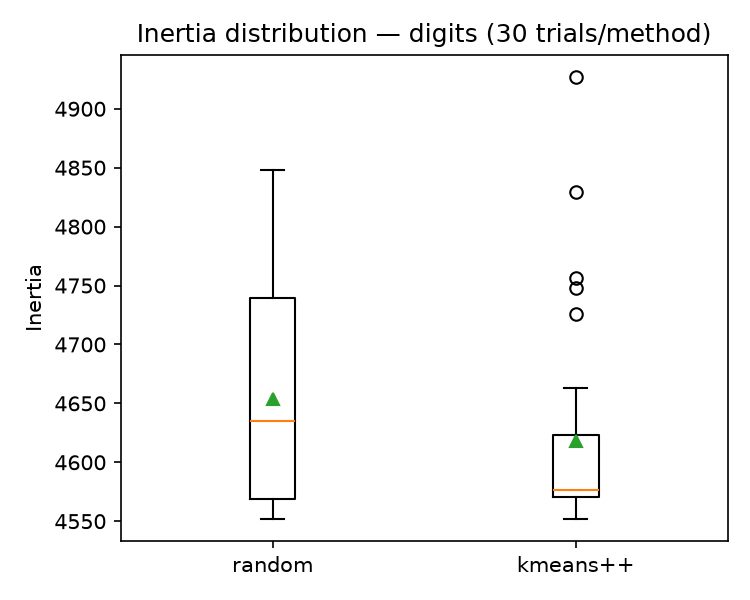
\includegraphics[width=0.6\textwidth]{outputs/figures/inertia_distribution_digits.png}
\caption{Inertia distribution over 30 trials per method, Digits dataset.}
\label{fig:digits_boxplot}
\end{figure}

\begin{figure}[H]
\centering
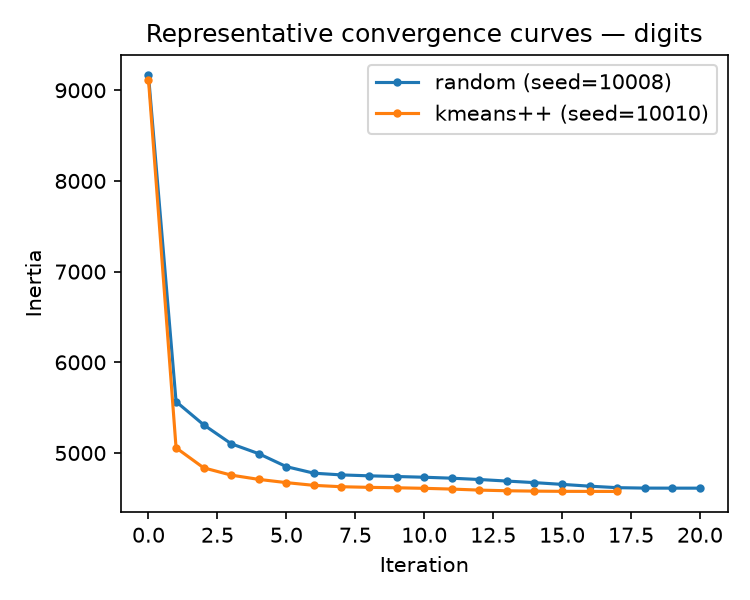
\includegraphics[width=0.6\textwidth]{outputs/figures/convergence_digits.png}
\caption{Representative convergence curves (median-inertia run per method), Digits dataset.}
\label{fig:digits_convergence}
\end{figure}

\subsection{Synthetic Dataset}
\label{sec:results_synthetic}

On the synthetic dataset the two methods reached essentially the same inertia values in
these trials: identical medians (2777.32) and identical IQRs (0.23) to the precision shown,
with means differing by only 0.02 out of roughly 2777 (Figure~\ref{fig:synth_boxplot}). We do
not draw conclusions about the number or shape of the underlying local optima from this; the
small residual difference could also partly reflect the stopping tolerance
(\texttt{tol=1e-4}) rather than a genuine gap in solution quality.
Figure~\ref{fig:synth_convergence} shows k-means++'s representative run starting from a
lower initial inertia (consistent with its spread-out seeding), though both curves converge to
essentially the same final value within about a dozen iterations. Figure~\ref{fig:synth_clusters}
shows the actual cluster assignments for the representative run of each method: both produce
four recognizable groups aligned with the generating regions, with visible overlap at the
shared boundaries, and centers
landing close to the true generating centers $(0,0)$, $(4,0)$, $(0,4)$, $(4,4)$.

\begin{figure}[H]
\centering
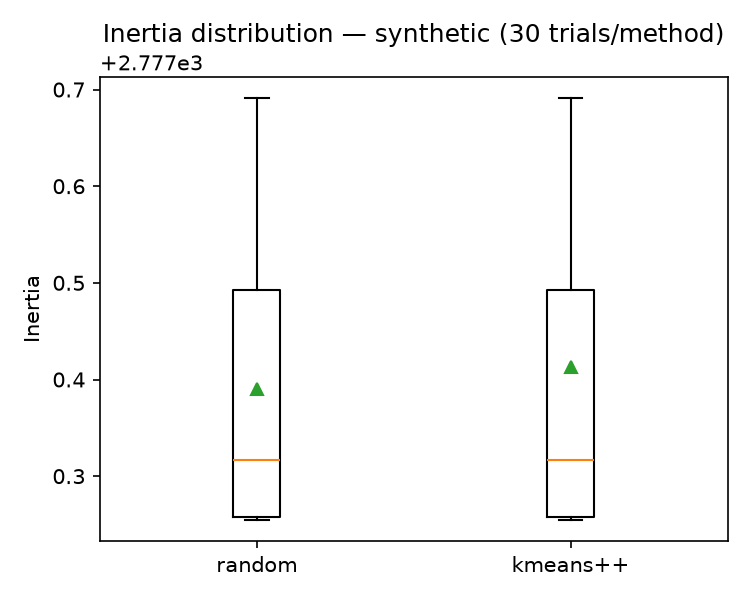
\includegraphics[width=0.6\textwidth]{outputs/figures/inertia_distribution_synthetic.png}
\caption{Inertia distribution over 30 trials per method, synthetic dataset. Note the
\texttt{+2.777e3} axis offset: the visible range spans less than 1 unit of inertia.}
\label{fig:synth_boxplot}
\end{figure}

\begin{figure}[H]
\centering
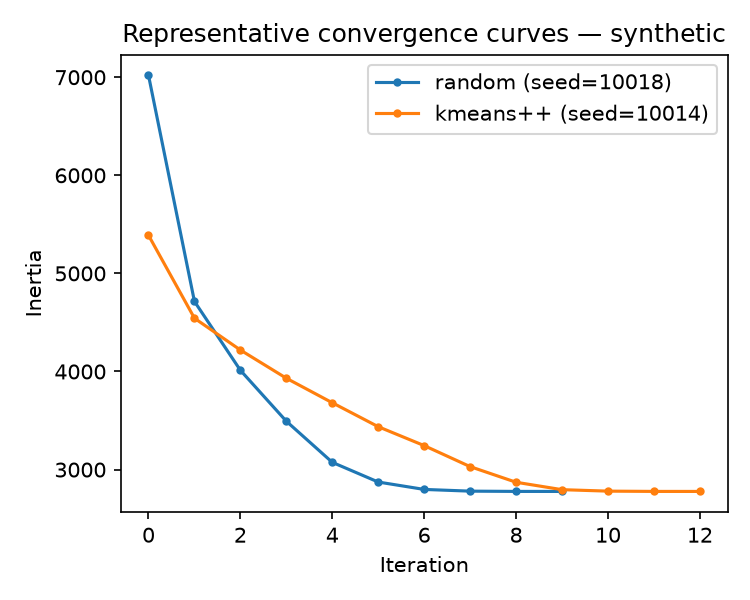
\includegraphics[width=0.6\textwidth]{outputs/figures/convergence_synthetic.png}
\caption{Representative convergence curves (median-inertia run per method), synthetic dataset.}
\label{fig:synth_convergence}
\end{figure}

\begin{figure}[H]
\centering
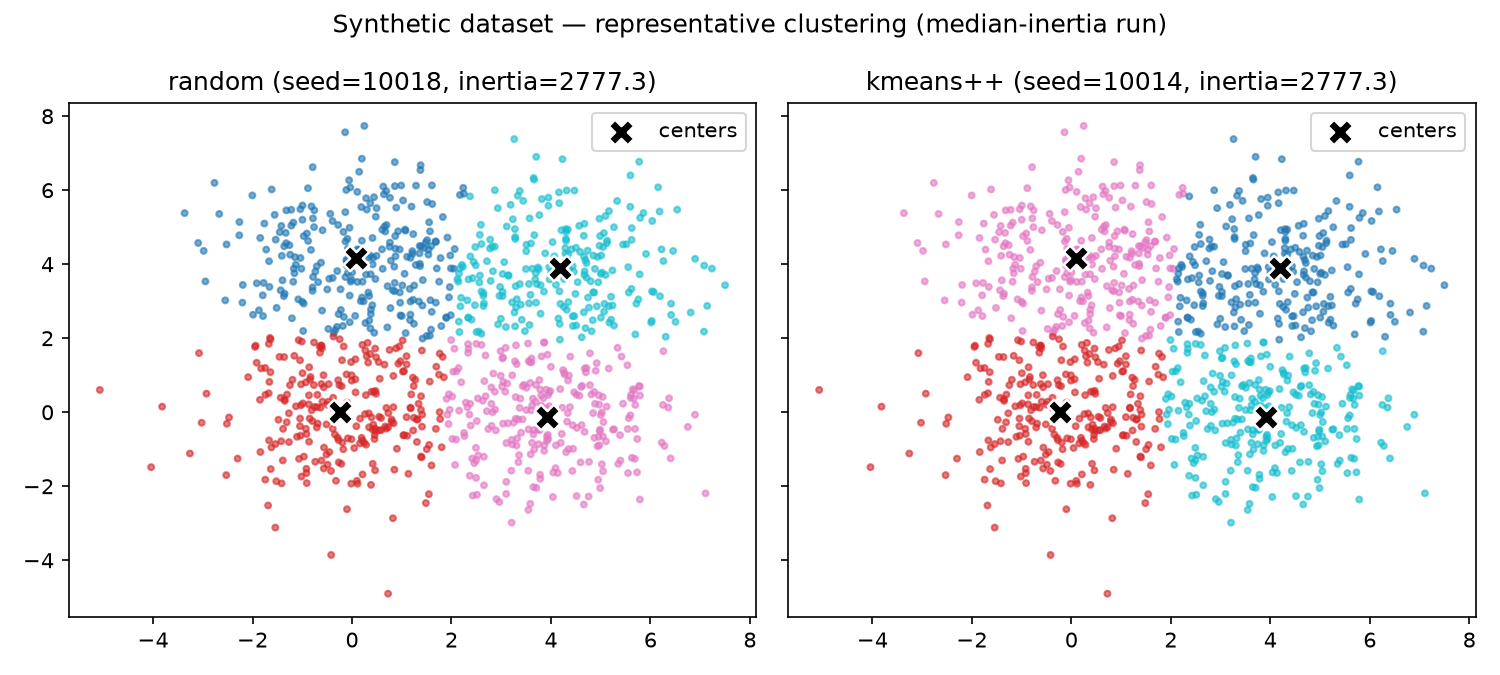
\includegraphics[width=\textwidth]{outputs/figures/synthetic_clusters.png}
\caption{Cluster assignments and final centers for the representative (median-inertia) run of
each method, synthetic dataset.}
\label{fig:synth_clusters}
\end{figure}

\subsection{Variability, Convergence, and Cross-Dataset Comparison}
\label{sec:crossdataset}

Every run converged under the relative-inertia stopping criterion, and none reached the
\texttt{max\_iter=300} cap; the largest iteration count observed was 31, for a k-means++ run
on Digits. Iteration counts were mildly higher, on average, for Digits than for the synthetic
data (Table~\ref{tab:iterations}); Digits is both higher-dimensional and structurally different
from the synthetic data (real pixel intensities versus generated Gaussians), and this
experiment cannot isolate dimensionality specifically as the cause of the higher iteration
counts. Within each dataset, the two methods used a comparable number of iterations, with
no large systematic gap.

Raw inertia values \emph{cannot} be compared directly between Digits and the synthetic
dataset: the two datasets differ in sample size ($n=1797$ vs.\ $n=1000$), dimensionality
($d=64$ vs.\ $d=2$), and number of clusters ($k=10$ vs.\ $k=4$), and Equation~\eqref{eq:inertia}
sums squared distances over $n$ points in $\mathbb{R}^d$, so its scale depends on all three
quantities as well as on the data's own spread. A lower absolute inertia on one dataset says
nothing about which dataset was ``better clustered.'' What \emph{can} be compared is the
qualitative behavior of the two methods: on the higher-dimensional, structurally different
Digits problem, k-means++ produced a tighter central inertia distribution than random --- a
lower median and a lower IQR --- while having a similar standard deviation and a worse
(higher) maximum; on the simpler, well-separated-by-design synthetic problem, initialization
made effectively no difference in these trials.

\section{Discussion: Positive and Negative Findings}
\label{sec:discussion}

\textbf{Positive.} On Digits, k-means++ produced a lower median inertia and a substantially
tighter IQR than random initialization: more of its runs landed near a good solution. All 120
runs converged well within the iteration budget, and our implementation's correctness checks
(reproducibility, shape/label validity, independently recomputed inertia, nearest-center
consistency, non-increasing inertia, and several edge cases) all passed.

\textbf{Negative and cautionary.} k-means++ did \emph{not} improve results on the synthetic
dataset in any visible way, and on Digits it still produced a worse-than-random outlier run
(max inertia 4927.28 vs.\ 4847.96 for random) and had a similar standard deviation to random,
so its improvement is a shift in the typical outcome, not a guarantee against poor runs. We
did not perform any formal statistical test (e.g., a rank-sum test on the two inertia
distributions), so we cannot and do not claim that the observed mean or median differences
are statistically significant. We also do not claim that k-means++ always outperforms random
initialization; our synthetic-dataset results are a direct counterexample within this
experiment.

\textbf{Limitations.} Only one synthetic configuration (fixed centers, spread, seed) was
tested, with no sweep over overlap, cluster count, or dimensionality. Thirty trials per group is
a moderate sample size; more trials or a formal hypothesis test would be needed for a
rigorous typical-case claim. Runtime was measured with a single timer call per run rather
than repeated, controlled benchmarking, so runtime differences should be read only
qualitatively. Only the Euclidean-distance $k$-means objective and two initialization schemes
were studied, with no comparison to other clustering algorithms or distance metrics. The
Digits dataset (64 dimensions, 1{,}797 samples) is smaller and lower-dimensional than MNIST;
it is used here as our chosen real-world, high-dimensional, multiclass substitute.

\section{Conclusion}
\label{sec:conclusion}

We implemented $k$-means with random and k-means++ initialization entirely from scratch in
NumPy, sharing one Lloyd loop, and compared them over 30 trials each on a synthetic 2D
dataset and the real-world Digits dataset. k-means++ produced a tighter central inertia
distribution on the higher-dimensional, structurally different Digits dataset --- lower IQR
and lower median inertia, with similar standard deviation and a worse maximum than random
--- while making essentially no difference on the simpler synthetic dataset, and it still
occasionally produced poor outlier runs on Digits. These results are directionally consistent
with the motivation behind k-means++ \cite{arthur2007kmeanspp} but, absent formal
significance testing, should be read as a qualitative, dataset-dependent pattern rather than a
general proof that careful seeding always helps.

\section{Reproducibility}
\label{sec:reproducibility}

The submitted repository (notebook, README, requirements, and all output files) is
self-contained. \texttt{README.md} documents installation and how to run the notebook
\texttt{clustering\_project.ipynb} from a fresh kernel with \texttt{QUICK\_MODE=False} to
reproduce the results in this report. All experiments use fixed, documented seeds, so
re-running the notebook reproduces the same inertia, iteration counts, and convergence
outcomes reported here.

\begin{thebibliography}{9}

\bibitem{smml_assignment5}
N.\ Cesa-Bianchi, E.\ Esposito, and L.\ Foscari.
\textit{Statistical Methods for Machine Learning --- Experimental Projects, A.Y.\ 2025/26}
(Assignment 5: Clustering and Initialization). Course assignment brief, University of Milan.

\bibitem{arthur2007kmeanspp}
D.\ Arthur and S.\ Vassilvitskii.
\textit{k-means++: The Advantages of Careful Seeding.}
In \textit{Proceedings of the Eighteenth Annual ACM-SIAM Symposium on Discrete Algorithms
(SODA)}, 2007.

\bibitem{sklearn_digits}
F.\ Pedregosa et al.
\textit{scikit-learn: Machine Learning in Python} --- \texttt{sklearn.datasets.load\_digits}
documentation. Journal of Machine Learning Research, 12:2825--2830, 2011.
\url{https://scikit-learn.org/stable/modules/generated/sklearn.datasets.load_digits.html}

\end{thebibliography}

\end{document}
